\documentclass[tikz]{standalone}
\usepackage{tikz}

\usetikzlibrary{positioning}
\usetikzlibrary{fit}
\usetikzlibrary{shapes}
\usetikzlibrary{arrows}

\tikzstyle{X} = [circle,fill=white,draw=black]
% Observed node
\tikzstyle{Y} = [X,fill=gray!25]
\tikzset{>={triangle 45}}

\begin{document}

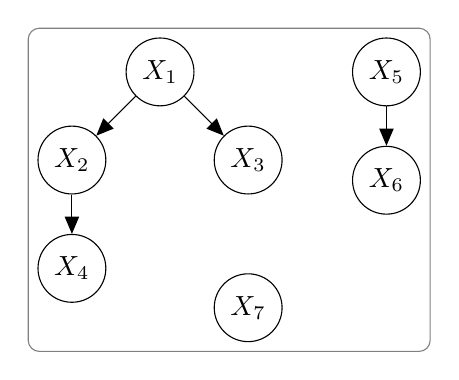
\begin{tikzpicture}
  \node [X] (n1) {$X_1$};    
  \node [X,below left=.5cm and .5cm of n1] (n2) {$X_2$};
  \node [X,below right=.5cm and .5cm of n1] (n3) {$X_3$};
  \node [X,below =.5cm  of n2] (n4) {$X_4$};
  
  \node [X,right=2cm  of n1] (n5) {$X_5$};
  \node [X,below=.5cm  of n5] (n6) {$X_6$};
  
  \node [X,below=1cm  of n3] (n7) {$X_7$};
  
	\draw [->] (n1) -- (n2) ;
	\draw [->] (n1) -- (n3) ;
	\draw [->] (n2) -- (n4) ;
	\draw [->] (n5) -- (n6) ;
	\node[draw=gray,rounded corners,fit=(n1)(n7)(n5)(n2)](r6){};
	%\node[draw=none,right=.5cm of r6](aa){\footnotesize Una foresta};
	%\draw [] (aa) -- (r6);
\end{tikzpicture}
\end{document}

%%% Local Variables:
%%% mode: latex
%%% TeX-master: t
%%% End:
